\documentclass[reqno, 10pt]{amsart}

%%%%%%%%%% Packages %%%%%%%%%%

\usepackage{amsmath,bbm,verbatim,wasysym,nicefrac,amssymb,braket}
%mathtools,appendix,soul,ulem,slashed,upgreek
\usepackage[protrusion=true, babel=true]{microtype}
\usepackage[english]{babel}
\usepackage[widespace]{fourier}
\usepackage[backrefs]{amsrefs}
\usepackage[margin=1in]{geometry}
\usepackage[onehalfspacing]{setspace}
\usepackage[pdfusetitle,pagebackref]{hyperref}
\numberwithin{equation}{section}                % must be called before cleveref
\usepackage[nameinlink,noabbrev]{cleveref}
\expandafter\def\csname ver@etex.sty\endcsname{3000/12/31}
\let\globcount\newcount
\usepackage{autonum}                            % must be called after cleveref
\usepackage[dvipsnames]{xcolor}
\usepackage{tikz}
\usetikzlibrary{quantikz}
\usepackage{subcaption}

%%%%%%%%%% align break fix %%%%%%%%%%

\allowdisplaybreaks[1]

%%%%%%%%%% Left/Right fix %%%%%%%%%%

\let\originalleft\left
\let\originalright\right
\renewcommand{\left}{\mathopen{}\mathclose\bgroup\originalleft}
\renewcommand{\right}{\aftergroup\egroup\originalright}

\def\({\mathopen{}\left(}
\def\){\right)\mathclose{}}

%%%%%%%%%% eqref fix %%%%%%%%%%

\makeatletter
\renewcommand*{\eqref}[1]{\hyperref[{#1}]{\textup{\tagform@{\ref*{#1}}}}}
\makeatother

%%%%%%%%%% oxford comma fix %%%%%%%%%%

\newcommand{\creflastconjunction}{, and\nobreakspace}

%%%%%%%%%% formula definitions %%%%%%%%%%

\newcommand*{\eqdef}{\mathrel{\vcenter{\baselineskip0.5ex \lineskiplimit0pt\hbox{.}\hbox{.}}}=}
\newcommand*{\defeq}{=\mathrel{\vcenter{\baselineskip0.5ex \lineskiplimit0pt\hbox{.}\hbox{.}}}}

%%%%%%%%%% Theorems/numbering %%%%%%%%%%

\newtheorem*{acknowledgment}{Acknowledgments}
\newtheorem{theorem}{Theorem}[section]
\newtheorem{proposition}[theorem]{Proposition}
\newtheorem{lemma}[theorem]{Lemma}
\newtheorem{corollary}[theorem]{Corollary}
\newtheorem{remark}[theorem]{Remark}
\newtheorem{definition}[theorem]{Definition}
\newtheorem{hypothesis}[theorem]{Hypothesis}
\newtheorem{example}[theorem]{Example}
\crefname{theorem}{Theorem}{Theorems}                 % label for Theorems
\creflabelformat{theorem}{#2{#1}#3}                   % label format for theorem
\crefname{main}{Main Theorem}{Main Theorems}          % label for the Main Theorems
\creflabelformat{main}{#2{#1}#3}                   % label format for main
\crefname{lemma}{Lemma}{Lemmas}                       % label for Lemmas
\creflabelformat{lemma}{#2{#1}#3}                     % label format for lem
\crefname{corollary}{Corollary}{Corollaries}          % label for Corollaries
\creflabelformat{corollary}{#2{#1}#3}                 % label format for cor
\crefname{ineq}{inequality}{inequalities}             % label for inequalities
\creflabelformat{ineq}{#2{\upshape(#1)}#3}               % label format for ineq
\crefname{diag}{diagram}{diagrams}             % label for diagrams
\creflabelformat{diag}{#2{\upshape(#1)}#3}               % label format for diag
\crefname{cond}{condition}{conditions}                % label for conditions
\creflabelformat{cond}{#2{#1}#3}                   % label format for cond
%\crefname{table}{Table}{Tables}                       % label for Tables
%\creflabelformat{table}{#2{\upshape(#1)}#3}              % label format for Tables
\crefname{hypothesis}{Hypothesis}{Hypotheses}            % label for Hypotheses
\creflabelformat{hypothesis}{#2{#1}#3}                % label format for Hypotheses
\crefname{remark}{Remark}{Remarks}                    % label for Remarks
\creflabelformat{remark}{#2{#1}#3}                    % label format for Remarks
\crefname{definition}{Definition}{Definitions}           % label for Definitions
\creflabelformat{def}{#2{#1}#3}                       % label format for 'def'

%%%%%%%%%% Blackboard %%%%%%%%%%

\def\id{\mathbbm{1}}
\def\cx{\mathbbm{C}}
\def\bG{\mathbbm{G}}
\def\rl{\mathbbm{R}}
\def\N{\mathbbm{N}}
\def\P{\mathbbm{P}}
\def\Z{\mathbbm{Z}}

%%%%%%%%%% CalligraPhics %%%%%%%%%%

\def\cA{\mathcal{A}}
\def\cB{\mathcal{B}}
\def\cC{\mathcal{C}}
\def\cD{\mathcal{D}}
\def\cE{\mathcal{E}}
\def\cF{\mathcal{F}}
\def\cG{\mathcal{G}}
\def\cH{\mathcal{H}}
\def\cI{\mathcal{I}}
\def\cK{\mathcal{K}}
\def\cL{\mathcal{L}}
\def\cM{\mathcal{M}}
\def\cN{\mathcal{N}}
\def\cO{\mathcal{O}}
\def\cP{\mathcal{P}}
\def\cR{\mathcal{R}}
\def\cS{\mathcal{S}}
\def\cT{\mathcal{T}}
\def\cU{\mathcal{U}}
\def\cV{\mathcal{V}}
\def\cW{\mathcal{W}}
\def\cZ{\mathcal{Z}}

%%%%%%%%%% Romans %%%%%%%%%%

\def\ad{\mathrm{ad}}
\def\Ad{\mathrm{Ad}}
\def\Aut{\mathrm{Aut}}
\def\coker{\mathrm{coker}}
\def\rd{\mathrm{d}}
\def\diag{\mathrm{diag}}
\def\dist{\mathrm{dist}}
\def\dom{\mathrm{dom}}
\def\Im{\mathrm{Im}}
\def\image{\mathrm{image}}
\def\index{\mathrm{index}}
\def\PU{\mathrm{PU}}
\def\rk{\mathrm{rk}}
\def\Re{\mathrm{Re}}
\def\Res{\mathrm{Res}}
\def\sign{\mathrm{sign}}
\def\SL{\mathrm{SL}}
\def\SO{\mathrm{SO}}
\def\spn{\mathrm{span}}
\def\Sym{\mathrm{Sym}}
\def\SU{\mathrm{SU}}
\def\supp{\mathrm{supp}}
\def\tr{\mathrm{tr}}

%%%%%%%%%% Other symbols (paper specific) %%%%%%%%%%

\def\qdict{\textsc{qdict}}
\def\QFT{\mathrm{QFT}}

%%%%%%%%%% Other formatting %%%%%%%%%%

\title{(Adaptive) Grover Fixed-point Search for QUBO Problems}
\date{\today}
\keywords{Grover Fixed-point Search, Quadratic Binary Optimization}
\subjclass[2020]{11E16, 68Q12, 81P65, 81P68}

\author{\'Akos Nagy}
\address[\'Akos Nagy]{BEIT Canada, Toronto, Ontario}
\email{\href{mailto:akos@beit.tech}{akos@beit.tech}}
\urladdr{\href{https://akosnagy.com/}{akosnagy.com}}

\author{Jaime Park}
\address[Jaime Park]{}
\email{\href{mailto:jaime.s.park@vanderbilt.edu}{jaime.s.park@vanderbilt.edu}}

\author{Cindy Zhang}
\address[Cindy Zhang]{}

\author{Atithi Acharya}
\address[Atithi Acharya]{}

\author{Alex Khan}
\address[Alex Khan]{}

\hypersetup{
   unicode        = true,
   pdffitwindow   = true,
   pdftoolbar     = false,
   pdfmenubar     = false,
   pdfstartview   = {FitH},
   hypertexnames  = true,
   colorlinks     = true,
   linkcolor      = black,
   citecolor      = black,
   filecolor      = black,
   urlcolor       = blue
}

\calclayout
\pagestyle{plain}
\clubpenalty = 10000
\widowpenalty = 10000
\setlength{\footskip}{20pt}

\hyphenation{}

\begin{document}

\begin{abstract}
   \emph{to be completed later...}
\end{abstract}

\maketitle

\section{Introduction}

Quadratic (Unconstrained) Binary Optimization problems provide some of the most interesting NP-Complete problems, such as cluster analysis, maximal graph cuts, or the Ising model. Approximation algorithms for such problems have been extensively studied for a long time both via classical methods and, more recently, using Quantum Computation {\color{red} add citations}.

\emph{to be completed later...}

\medskip

\subsection{Results:}

\smallskip

\subsection*{Organization of the paper:} In \Cref{sec:qubos_and_qdicts}, we introduce the two central notions of the paper; QUBO problems and Quantum Dictionaries. In \Cref{sec:quad}, we provide an outline of the construction of \cite{gilliam_grover_2021} of the oracle for QUBOs and in \Cref{sec:xor_basis} we give our modified design. \emph{to be completed later...}

\smallskip

\subsection*{Acknowledgment:} We are grateful to Amazon Web Services and QLab for providing credits to access IonQ's QPUs. We also thank to Constantin Gonciulea for providing feedback on an earlier version of the work and QuForce.org for bringing the authors together for the project. \Cref{sec:grover_for_qubo} introduces the Grover Fixed-point search for QUBOs.

\bigskip

\section{(Polynomial Unconstrained) Binary Optimization and Quantum Dictionaries}
\label{sec:qubos_and_qdicts}

For the rest of the paper, $\Z_2^n$ denotes the space of length-$n$ bitstrings. If $x \in [0, 2^n - 1] \cap \Z$ and its binary representation if $x = \overline{x_0 x_1 \ldots x_{n - 1}} = \sum_{i = 0}^{n - 1} x_i 2^{n - 1 - i}$, then $\ket{x}_n \eqdef \ket{x_0} \ket{x_1} \ldots \ket{x_{n - 1}}$, and for an arbitrary $x \in \Z$, $\ket{x}_n = \ket{\bar{x}}_n$, where $x \equiv_{\mod n} \bar{x} \in [0, 2^n - 1] \cap \Z$. We also drop the subscript $n$, when it is unambiguous. Given a function $f : \Z_2^n \rightarrow \rl$, the associated (Unconstrained) Binary Optimization problem is the task of finding an element $x \in \Z_2^n$ such that $f (x)$ is maximal. Note that every binary function is polynomial, which can be seen by simple dimension count.

Many interesting Binary Optimization problems, such as finding maximal graph cuts or the Max $2$-SAT problems are quadratic, and most of the contemporary research centers around Quadratic Unconstrained  Binary Optimization (QUBO) problems.

\medskip

The first main contribution of the paper is an oracle design for QUBO problems. More concretely, we construct encoding operators of \emph{quantum dictionaries}, as introduced in \cite{gilliam_foundational_2021}. Such oracles have applications, for example, in Grover type algorithms and threshold QAOA \cite{golden_threshold_2021}. While such designs have already existed, cf. \cite{gilliam_grover_2021}, ours has better circuit depth, gate count, and CNOT count. Thus, they are simultaneously faster and more noise-resistant.

Briefly, the quantum dictionary, corresponding to a function (thought of as a classical dictionary), $F: \dom \( F \) \rightarrow \Z_2^d$, where $\dom \( F \) \subseteq \Z_2^n$, is the following quantum state on $n + d$ qubits:
\begin{equation}
   \ket{\qdict \( F \)} \eqdef \tfrac{1}{\sqrt{\left| \dom \( F \) \right|}} \sum\limits_{x \in \dom \( F \)} \ket{x}_n \ket{F (x)}_d.
\end{equation}

An integer-valued function $f : \Z_2^n \rightarrow \Z$ canonically determines a quantum dictionary via first defining $F (x)$ to be the digits of $f (x)$, then setting, by a slight abuse of notation, $\ket{\qdict \( f \)} = \ket{\qdict \( F \)}$. Let us handle signs via the ``Two's complement'' convention, in particular, a binary number $y_0 y_1 \ldots y_{d - 1}$ is negative exactly when $y_0 = 1$. In fact, every quantum dictionary can be realized in this a way.

\smallskip

We construct the above-mentioned encoding oracles in two steps. First, we outline a modified version of the encoding operator given in \cite{gilliam_grover_2021} that is convenient to encode quadratic polynomials. Then we show that quadratic polynomial can be expressed in a basis of functions that can be more efficiently encoded.

\medskip

\subsection{Quadratic encoder}
\label{sec:quad}

Let $I \subseteq \{ 1, 2, \ldots, n - 1 \}$ and $p_I (x) \eqdef x_{i_1} x_{i_2} \cdots x_{i_j}$ be an arbitrary monomial and consider a quantum circuit with $n + d$ qubits. Following \cite{gilliam_grover_2021}, we construct an oracle that sends $\ket{x}_n \ket{0}_d$ to $\ket{x}_n \ket{p_I (x)}_d$, for any $x \in \Z_2^n$.

Let us make two definitions: Let $\QFT_d$ be the Quantum Fourier Transform on $m$ qubits, that is for any $- 2^{d - 1} \leqslant y < 2^{d - 1}$, we have
\begin{equation}
   \QFT_d \ket{y}_d = 2^{- \frac{d}{2}} \sum\limits_{z = - 2^{d - 1}}^{2^{d - 1} - 1} e^{\frac{2 \pi y z}{2^d} i} \ket{z}_d.
\end{equation}
Then
\begin{equation}
   \QFT_d^\dagger \ket{z}_d = 2^{- \frac{d}{2}} \sum\limits_{y^\prime = - 2^{d - 1}}^{2^{d - 1} - 1} e^{- \frac{2 \pi y^\prime z}{2^d} i} \ket{y^\prime}_d.
\end{equation}
Now let $\cP_d (k)$ be the following $m$-qubit gate
\begin{equation}
   \begin{quantikz}
      \lstick{$\ket{z_0}$} \qw  &  \gate{\textsc{phase} \( \pi k \)} & \qw \rstick{$e^{\frac{2 \pi i}{2^d} k z_0 2^{d - 1}} \ket{z_0}$} \\
      \vdots \\
      \lstick{$\ket{z_j}$} \qw  &  \gate{\textsc{phase} \( \tfrac{2 \pi k}{2^{j + 1}} \)} & \qw \rstick{$e^{\frac{2 \pi i}{2^d} k z_j 2^{d - j - 1}} \ket{z_j}$} \\
      \vdots \\
      \lstick{$\ket{z_{d - 1}}$} \qw  &  \gate{\textsc{phase} \( \tfrac{2 \pi k}{2^d} \)} & \qw \rstick{$e^{\frac{2 \pi i}{2^d} k z_{d - 1}} \ket{z_d}$}
   \end{quantikz}   
\end{equation}
Thus $\cP_d \( k \) \ket{z}_d = e^{\frac{2 \pi k z}{2^d} i} \ket{z}_d$.

Now we can prove a well-known lemma. {\color{Red} citation needed}

\begin{lemma}
   \label{lemma:quantum_adder}
   For any $- 2^{d - 1} \leqslant y < 2^{d - 1}$ and $k \in \Z$ we have
   \begin{equation}
      \QFT_d^\dagger \circ \cP_d \( k \) \circ \QFT_d \ket{y}_d = \ket{y + k}.
   \end{equation}
\end{lemma}

\begin{proof}
   First we compute
   \begin{align}
      \cP_d \( k \) \circ \QFT_d \ket{y}_d  &= \cP \( k \) \( 2^{- \frac{d}{2}} \sum\limits_{z = - 2^{d - 1}}^{2^{d - 1} - 1} e^{\frac{2 \pi y z}{2^d} i} \ket{z}_d \) \\
         &= 2^{- \frac{d}{2}} \sum\limits_{z = - 2^{d - 1}}^{2^{d - 1} - 1} e^{\frac{2 \pi y z}{2^d} i} \cP \( k \) \ket{z}_d \\
         &= 2^{- \frac{d}{2}} \sum\limits_{z = - 2^{d - 1}}^{2^{d - 1} - 1} e^{\frac{2 \pi \( y + k \) z}{2^d} i} \ket{z}_d \\
         &= \QFT_d \ket{y + k},
   \end{align}
   hence
   \begin{equation}
      \QFT_d^\dagger \circ \cP \( k \) \circ \QFT_d \ket{y}_d = \ket{y + k}.
   \end{equation}
\end{proof}

By \Cref{lemma:quantum_adder} it is immediate that
\begin{equation}
   \begin{quantikz}
      \lstick{$\ket{x}_n$}   & \qw  & \qw             & \qw & \ctrl{1}                & \qw & \qw                    & \qw \rstick{$\ket{x}_n$} \\
      \lstick{$\ket{0}_d$}   & \qw  & \gate{\QFT_d}   & \qw & \gate{C_I \cP \( 1 \)}  & \qw & \gate{\QFT_d^\dagger}  & \qw \rstick{$\ket{p_I (x)}_d$}
   \end{quantikz}
\end{equation}
where $C_I$ means control by the qubits $i_1, i_2, \ldots i_j$.

Finally, to create the full quantum dictionary, $\ket{\qdict \( f \)}$, we need to pre-compose an oracle, call $U$, for which we have
\begin{equation}
   U \ket{0}_n = \tfrac{1}{\sqrt{\left| \dom \( f \) \right|}} \sum\limits_{x \in \dom \( f \)} \ket{x}_n.
\end{equation}
If $\dom \( f \) = \Z_2^n$, then $U = H^{\otimes n}$.
\begin{example}
   Let $n = d = 2$ and $f (x) = x_0 x_1$. Now the encoder oracle takes the form
   \begin{equation}
      \begin{quantikz}
         \lstick{$\ket{0}$}   & \qw  & \gate[2]{U}             & \qw & \ctrl{1}    & \qw & \ctrl{1}                                      & \qw & \qw \rstick[4]{$\ket{\qdict \( f \)}$} \\
         \lstick{$\ket{0}$}   & \qw  &                         & \qw & \ctrl{1}                                                                                                                                                                       & \qw & \ctrl{2}                                      & \qw                      & \qw \\
         \lstick{$\ket{0}$}   & \qw  & \gate[2]{H^{\otimes 2}} & \qw & \gate{\textsc{phase} \( \pi \)} \gategroup[2, steps=3, style={dashed, rounded corners, fill=blue!20}, background, label style={label position=below, anchor=north, yshift=-1em}]{$\cP \( 1 \)$}                                                                                                                                                & \qw & \qw                                           & \gate[2]{\QFT_2^\dagger} & \qw \\
         \lstick{$\ket{0}$}   & \qw  &                         & \qw & \qw                                                                                                                                                                            & \qw & \gate{\textsc{phase} \( \nicefrac{\pi}{2} \)} &                          & \qw,
      \end{quantikz}
   \end{equation}
   where we used that $\QFT_d \ket{0}_d = H^{\otimes d} \ket{0}_d$.
\end{example}

\smallskip

For the rest of the paper we assume that $\dom \( f \) = \Z_2^n$ and use $U = H^{\otimes n}$. Furthermore, since $\QFT_d \ket{0}_d = H^{\otimes m} \ket{0}_d$, we can replace $\QFT_d$ with $H^{\otimes d}$ in the oracle, as the latter has depth $1$ and uses only single-qubit gates.

Let $\P_n$ be the power set of $\{ 0, 1, \ldots, n - 1 \}$. Now, for an arbitrary polynomial,
\begin{equation}
   f (x) = \sum\limits_{I \in \P_n} A_I x^I,
\end{equation}
and $d \in \Z_+$ large enough so that all values of $f$ can be digitized on $m$ bits, we have that
\begin{equation}
   \begin{quantikz}
      \lstick{$\ket{0}_n$}   & \qw              & \gate[2]{H^{\otimes (n + d)}}        & \qw & \ctrl{1} \gategroup[2, steps=1, style={dashed, rounded corners, fill=blue!20}, background, label style={label position=below, anchor=north, yshift=-1em}]{\tiny{one for each $I = \left\{ i_1, i_2, \ldots, i_{|I|} \right\} \in \P_n$, controlled by qubits $x_{i_1}, x_{i_2}, \ldots, x_{i_{|I|}}$}}                    & \qw \ \ldots \ & \qw & \qw                   & \qw \rstick[2]{$\ket{\qdict \( f \)}$} \\
      \lstick{$\ket{0}_d$}   & \qw  & & \qw & \gate{\cP \( A_I \)}   & \qw \ \ldots \ & \qw & \gate{\QFT_d^\dagger} & \qw
   \end{quantikz}
\end{equation}

\medskip

\subsection{New basis for quadratic polynomials and the new oracle design}
\label{sec:xor_basis}

We motivate the idea of the new basis by outlining it in the $n = 2$ case.

\smallskip

Note first that, since $x_i^2 = x_i$ for binary variables, we have that $x_0 x_1 = \tfrac{1}{2} \( x_0 + x_1 - \( x_0 - x_1 \)^2 \)$. Now $\( x_0 - x_1 \)^2$ is also a binary variable, in fact, $\( x_0 - x_1 \)^2 = x_0 \textnormal{ XOR } x_1$. Now let $f$ be a generic polynomial, $f \( x_0, x_1 \) = A_\emptyset + A_0 x_0 + A_1 x_1 + A_{01} x_0 x_1$. Since we are interested in finding the maximum of $f$, we can assume, without any loss of generality, that $f (0, 0) = A_\emptyset = 0$. By generic, we mean that $0 \notin \{ A_0, A_1, A_{01} \}$. Using $d$ digits, we need $2 d$ CNOT gates for each linear terms and $6 d$ CNOT gates for the quadratic term, thus a total of $10 d$ CNOT gates (not counting the CNOT gates in $\QFT_d^\dagger$). However, we can rewrite $f$ as
\begin{align}
   f \( x_0, x_1 \)  &= A_0 x_0 + A_1 x_1 + A_{01} x_0 x_1 \\
                     &= \overbrace{\( A_0 + \tfrac{1}{2} A_{01} \)}^{\widetilde{A}_0 \eqdef} x_0 + \overbrace{\( A_1 + \tfrac{1}{2} A_{01} \)}^{\widetilde{A}_1 \eqdef} x_1  + \overbrace{\( - \tfrac{1}{2} A_{01} \)}^{\widetilde{A}_{01} \eqdef} \( x_0 - x_1 \)^2,
\end{align}
and note that the last term can be implemented as
\begin{equation}
   \begin{quantikz}
      \lstick{$\ket{x_0}$} \qw & \ctrl{1}   & \qw                  & \ctrl{1}              & \qw \\
      \lstick{$\ket{x_1}$} \qw & \targ{}    & \ctrl{1}             & \targ{}               & \qw \\
      \lstick{$\ket{y}_d$} \qw & \qw        & \gate{\cP \( 1 \)}   & \qw                   & \qw
   \end{quantikz}
\end{equation}
which now has CNOT count only $2 + 2d$. Thus the whole oracle (for arbitrary $f$) can be realized as
\begin{equation}
   \begin{quantikz}
      \lstick{$\ket{x_0}$} \qw & \gate[3]{H^{\otimes (2 + d)}}  & \ctrl{2}                                   & \qw                                        & \ctrl{1}   & \qw                                    & \ctrl{1}              & \qw \rstick[3]{$\ket{\qdict \( f \)}$} \\
      \lstick{$\ket{x_1}$} \qw &                                & \qw                                        & \ctrl{1}                                   & \targ{}    & \ctrl{1}                               & \targ{}               & \qw \\
      \lstick{$\ket{0}_d$} \qw &                                & \gate{\cP \( \widetilde{A}_0 \)}   & \gate{\cP \( \widetilde{A}_1 \)}   & \qw        & \gate{\cP \( \widetilde{A}_{01} \)}   & \gate{\QFT_d^\dagger} & \qw
   \end{quantikz}
\end{equation}
making the new CNOT count for the whole oracle to be (at most) $2 + 6d$, again, not counting the CNOT gates in $\QFT_d^\dagger$. In fact, the only time the two counts equal is when $A_0 = A_1 = 0$, $A_{01} \neq 0$, and $d = 1$.

\smallskip

For a general, $n$-bit, quadratic polynomial, given by a symmetric, real, $n$-by-$n$ matrix, $Q$ via
\begin{equation}
   f \( x_0, x_1, \ldots, x_{n - 1} \) = x^T Q x = \sum\limits_{i = 0}^{n - 1} Q_{ii} x_i + 2 \sum\limits_{i = 0}^{n - 2} \sum\limits_{j = i + 1}^{n - 1} Q_{ij} x_i x_j,
\end{equation}
we have that if $q_i = \sum\limits_{j = 0}^{n - 1} Q_{ij}$ is the sum of the $i^{\mathrm{th}}$ row, then
\begin{align}
   f \( x_0, x_1, \ldots, x_{n - 1} \) = \sum\limits_{i = 0}^{n - 1} q_i x_i - \sum\limits_{i = 0}^{n - 2} \sum\limits_{j = i + 1}^{n - 1} Q_{ij} \( x_i - x_j \)^2.
\end{align}
The addition of a quadratic term, $x_i x_j$, in the oracle design of \cite{gilliam_grover_2021} is implemented via a $2$-controlled $\cP$-gate, whereas the addition of the term, $\( x_i - x_j \)^2$, in our construction is implemented via a $1$-controlled $\cP$-gate and $2$ additional CNOT gates, which is generally more economical both in terms of circuit depth and entangling gate counts. In particular, when decomposed to single-qubit gates and CNOT gates, the former design needs $8d$ for each $2$-controlled $\cP$-gate, while the latter requires only $2 + 2d$ CNOT gates. Thus the total CNOT counts for a generic quadratic polynomial are $n \( 2 d \) + \tfrac{n \( n - 1 \)}{2} \( 8 d \) = \( 4 n^2 - 2 n \) d$ and $n \( 2 d \) + \tfrac{n \( n - 1 \)}{2} \( 2 + 2 d \) = \( d + 1 \) n^2 + \( d - 1\) n$, respectively, which is an approximately fourfold improvement. Since up to $d$ terms can be digitized in parallel, the time complexity of the oracle is $O \( n^2 \)$, as long as $d = o \( n \)$.

\smallskip

\begin{remark}
   In the case a single, quadratic monomial and $d = 1$, there is no advantage; in fact, in this case, our construction is just the well-known $2$-controlled phase gate from \cite{nielsen_quantum_2010}*{Figure~4.8}. Using this observation and a bit more work, one can also show that our construction is never worse (in terms of gate count, CNOT count, or gate circuit depth), than that of \cite{gilliam_grover_2021}.

   A further generalization of this construction to higher degree polynomials is also currently being prepared by the authors.
\end{remark}

\bigskip

\section{Grover Fixed-point search for QUBO}
\label{sec:grover_for_qubo}

Grover Fixed-Point Search (GFPS) \cite{yoder_fixed_2014} is a variant of Grover's search algorithm that retains the original version query complexity while does not suffer from the souffl\'e problem (more on these below). In this section we introduce the algorithm, show how our oracle design from \Cref{sec:xor_basis} can be used to implement GFPS for QUBO problems, and argue that this method is better suited for an adaptive optimizer algorithm than the original.

\smallskip

As opposed to Grover's algorithm, where the only input is the set of \emph{good} (or \emph{target}) configurations, $T \subset \Z_2^n$, the GFPS algorithm requires an additional one, that can be chosen to be either the target probability/amplitude or the query complexity. The target probability is the probability of finding the system in a good state after running the circuit. The price of this flexibility (and of the elimination of half of the souffl\'e problem) is that one needs to implement not only a pair of oracles, but two families of them, call $S_s \( \alpha \)$ and $S_t \( \beta \)$ (where the subscripts refer to the \emph{start} and \emph{target} states, and $\alpha, \beta$ are real parameters), with the following properties: let us fix gauge so that, for some $\lambda \in \( 0, 1 \)$, we can write
\begin{align}
   \ket{s}  &= \sqrt{\lambda} \ket{t} + \sqrt{1 - \lambda} \ket{\overline{t}}, \\
   \ket{t}  &= \sqrt{\lambda} \ket{s} + \sqrt{1 - \lambda} \ket{\overline{s}},
\end{align}
where $\braket{t | \overline{t}} = \braket{s | \overline{s}} = 0$. Then
\begin{align}
   S_s \( \alpha \) \( A \ket{s} + B \ket{\overline{s}} \)  &= e^{i \alpha} A \ket{s} + B \ket{\overline{s}}, \\
   S_t \( \beta \) \( D \ket{t} + C \ket{\overline{t}} \)   &= e^{i \beta} C \ket{t} + D \ket{\overline{t}}.
\end{align}
Let $G \( \alpha, \beta \) \eqdef S_s \( \alpha \) S_t \( \beta \)$. Once in possession of such oracles and a target probability $P \in \( 0, 1 \)$, the main result of \cite{yoder_fixed_2014} can be summarized as follows: for any $\mu \in \( 0, \lambda \right]$ large enough, there exists $l = l \( P, \mu \) \in \Z_+$ and $\delta = \delta_{P, \mu} \in \( 0, 1 \)$, such that if, for all $j \in \{ 1, \ldots, l \}$, we set
\begin{align}
   \alpha_j &\eqdef 2 \mathrm{arccot} \( \tan \( \tfrac{2 \pi j}{2 l + 1} \) \tanh \( \tfrac{\mathrm{arccosh} \( \nicefrac{1}{\delta} \)}{2 l + 1} \) \), \\
   \beta_j  &\eqdef \alpha_{l - j + 1},
\end{align}
then
\begin{equation}
   P_{\mathrm{success}} \eqdef \left| \left\langle t \middle| G \( \alpha_l, \beta_l \) \cdots G \( \alpha_1, \beta_1 \) \middle| s \right\rangle \right|^2 \geqslant P.
\end{equation}
Moreover, $l, \delta$ can be explicitly computed (see next section).

\smallskip

We implement $S_s \( \alpha \)$ and $S_t \( \beta \)$ in straightforward ways. If $U_s$ is the state preparation oracle, that is, $\ket{s} = U_s \ket{0}$, and $\mathrm{MCP}_n \( \alpha \)$ is the $(n - 1)$-controlled phase gate on $n$ qubits, then
\begin{equation}
   S_s \( \alpha \) = U_s \mathrm{MCP}_n \( \alpha \) U_s^\dagger, \label{eq:diffuser}
\end{equation}
works. Note that $\mathrm{MCP}_n$ can be implemented with $O \( n^2 \)$ CNOT gates and circuit depth, and no ancillas; cf. \cite{linear_dasilva_2022}.

In general, the implementation of $S_t \( \beta \)$ is case specific. In the case of an instance of a QUBO problem, let $T \eqdef \{ x \in \Z_2^n | f(x) < 0 \}$. Now the results of \Cref{sec:quad,sec:xor_basis} can be immedately used to get an oracle, $U_t$, on $n + 1$ qubits, such that for all $x \in \Z_2^n$ and $y \in \Z_2$, we have
\begin{equation}
   U \ket{x} \ket{y} = \left\{ \begin{array}{ll} \ket{x} \ket{y \oplus 1}, & \mbox{if } x \in T, \\ \ket{x} \ket{y}, & \mbox{if } x \notin T, \end{array} \right.
\end{equation}
where the last qubit, $\ket{y}$, is the first ancilla of the original oracle. Now
\begin{equation}
   \begin{quantikz}
      \lstick{$\ket{x}$} \qw & \gate[2]{U_t} \gategroup[2, steps=3, style={dashed, rounded corners, fill=blue!20}, background, label style={label position=below, anchor=north, yshift=-1em}]{$S_t \( \beta \)$} & \qw & \gate[2]{U_t} & \qw \rstick[2]{$e^{i \beta} \ket{x} \ket{y}$} \\
      \lstick{$\ket{y}$} \qw & & \gate{\textsc{phase} \( \beta \)} & & \qw
   \end{quantikz}
\end{equation}
works for $S_t \( \beta \)$, if the $(n + 1)^{\mathrm{st}}$ qubits is a clean ancilla kept in $\ket{0}$ before and after the usage of the oracle. Since QFT can be implemented on $d$ qubits use $O \( d^2 \)$ CNOT gates, the (worst case) CNOT count of $U_t$ is $O \( n^2 \)$, as long as $d = O \( n^2 \)$.

\smallskip

\begin{remark}
   \label{remark:graphcuts}
    In the case when $f$ is the cut function of a simple, unoriented, and undirected graph, with $n$ vertices and $m$ edges, GFPS can be implemented on $n + O \( \log (m) \)$ qubits, with gate count being $O \( m \log (m) \)$, and circuit depth of $O \( m \)$.
\end{remark}

\bigskip

\subsection{Time complexity}
\label{sec:time}

In order to understand the time-complexity of GFPS for QUBO problems, we need two know three things:
\begin{enumerate}

   \item The query complexity, $l$.

   \item The complexity of the diffusion operator, $S_s \( \alpha \)$. Let us call this complexity $C_s$.

   \item The complexity of the operator, $S_t \( \beta \)$. Let us call this complexity $C_t$.

\end{enumerate}

The time complexity is then $l \( C_s + C_t \)$. From \cite{yoder_fixed_2014}, we know that $l \approx \tfrac{\ln \( 2 / \delta \)}{\sqrt{\mu}}$ is sharp. By \cref{eq:diffuser}, we see that $C_s$ is the same as the time complexity of the $\mathrm{MCP}_n \( \alpha \)$ gate. By \cite{linear_dasilva_2022}, we get that $C_s \leqslant O \( n^2 \)$ (and this is applies to both single qubit and CNOT gate counts). Finally, by the argument of the previous section, $C_t = O \( n^2 \)$ as well. This yields, for a fixed $\delta$, that the total time complexity if $O \( \mu^{- \frac{1}{2}} n^2 \)$. Note that we still have the choice of the number $\mu \in \( 0, \lambda \right]$ that we discuss in the next section.

\begin{remark}
   In the case of maximal graph cuts, we have already seen in \Cref{remark:graphcuts} we have already seen that the complexity becomes $C_t = O \( m \) \leqslant O \( n^2 \)$, and thus the complexity of GFPS is $O \( \mu^{- \frac{1}{2}} \( n^2 + m \ln(m) \) \)$.
\end{remark}

\bigskip

\section{Adaptive Search}
\label{sec:adaptive}

As mentioned in the previous section, the choice of $\mu$ is problematic; it needs to be at most $\lambda \in \( 0, 1 \)$, the ratio of marked configurations to all configurations (or, more precisely, the tunneling amplitude between the initial state and the target state), but $\lambda$ is not known. The ideal choice would be $\mu = \lambda$, but $\lambda$ is not known. It can be, partially, remedied as follows: Using repeated runs with $\lambda_k = \lambda_0 2^{- k}$ with $k = 1, 2, \ldots$, we can get under $\lambda$ while not increasing the big-$O$ time complexity of the algorithm. Furthermore, note that so far we only implemented a search algorithm that finds negative values of a(n integer-valued) QUBO problem. For any given $y \in \Z$, we can repeat the algorithm with the polynomial $y - f(x)$, making the set of marked states to be $T_y \eqdef \{ x \in \Z_2^n | f(x) > y \}$. Since our goal is not just to find configurations, $x$, with values, $f(x)$, above a certain threshold, but rather to find configurations with as high values as possible, we regard $y$ as another parameter.

\smallskip

We propose the following adaptive (quantum--classical hybrid) method: Let us assume that we are given an instance of a QUBO problem and a time threshold $t_{\max} > 0$, and our goal is to find a configuration with the highest value under $t_{\max}$ time.

Set $t \eqdef 0$, $\lambda_{0, \mathrm{i}} \eqdef \tfrac{1}{2}$, choose $x_0 \in Z_2^n$ randomly, and set $y_0 \eqdef f \( x_0 \)$. While $t < t_{\max}, \: (k \in \Z_+)$, do
\begin{itemize}
   \item[] Given $y_k, \lambda_{k, \mathrm{initial}}$, use the above method to search for $x_{k + 1}$ with $f \( x_{k + 1} \) > y_k$, while in each round incrementing $t$ by the query complexity $l$.
   
   \item[] If $x_{k + 1}$ is found before termination: Let $\lambda_{k, \mathrm{final}} > 0$ be the parameter of this search, and set $y_{k + 1} \eqdef f \( x_{k + 1} \)$, $\lambda_{k + 1, \mathrm{initial}} \eqdef \lambda_{k, \mathrm{final}}$.
\end{itemize}
Output the last configuration.

\smallskip

\begin{remark}
   The parameter $\delta$, that is approximately the square root of the failure probability, is assumed to be small, but not changed throughout the iterations. Allowing $\delta$ to vary is another potential direction of improvement.
\end{remark}

\bigskip

\section{Experiments on IonQ's Quantum Computers}
\label{sec:experiments}

\subsection{Oracle testing:} The marker oracle, $U_t$, was tested on IonQ's Aria $2$ QPU. We used $9$ qubits ($5$-bit QUBO with $4$ ancillas) with $5000$ shots. The matrix of the quadratic form was
\begin{equation}
   Q = \begin{pmatrix}
         2 & - 1 & 0 & - 1 & 0 \\
         - 1 & 1 & 0 & 0 & 0 \\
         0 & 0 & 2 & 0 & - 1 \\
         - 1 & 0 & 0 & 2 & 0 \\
         0 & 0 & - 1 & 0 & 2
      \end{pmatrix},
\end{equation}
with threshold $y = 5$ that is, in fact, the maximum. Out of the $2^5 = 32$ configurations only $3$ equal to the threshold, thus $\lambda = \tfrac{3}{32}$. We index the configurations according to the numerical value they represent in base $2$. The experimental results are given in \Cref{table:oracle}.
\begin{table}[ht]
   \begin{tabular}{|l|c|c|c||l|c|c|c|}
      \hline
      index & $y - f (x)$ & not marked & marked & index & $f (x) - y$ & not marked & marked \\
      \hline
      1 & 3 & {\color{ForestGreen} 1.68\%} & {\color{Red} 0.36\%} & 17 & 1 & {\color{ForestGreen} 1.06\%} & {\color{Red} 0.26\%} \\
      2 & 4 & {\color{ForestGreen} 3.18\%} & {\color{Red} 0.52\%} & 18 & 2 & {\color{ForestGreen} 1.04\%} & {\color{Red} 0.30\%} \\
      3 & 4 & {\color{ForestGreen} 4.08\%} & {\color{Red} 0.86\%} & 19 & 2 & {\color{ForestGreen} 2.02\%} & {\color{Red} 0.48\%} \\
      4 & 3 & {\color{ForestGreen} 2.16\%} & {\color{Red} 0.68\%} & 20 & 3 & {\color{ForestGreen} 3.90\%} & {\color{Red} 0.78\%} \\
      5 & 1 & {\color{ForestGreen} 2.02\%} & {\color{Red} 0.40\%} & 21 & 1 & {\color{ForestGreen} 2.30\%} & {\color{Red} 0.36\%} \\
      6 & 2 & {\color{ForestGreen} 1.34\%} & {\color{Red} 0.36\%} & 22 & 2 & {\color{ForestGreen} 3.42\%} & {\color{Red} 0.58\%} \\
      7 & 2 & {\color{ForestGreen} 2.90\%} & {\color{Red} 0.32\%} & 23 & 2 & {\color{ForestGreen} 4.54\%} & {\color{Red} 0.34\%} \\
      8 & 3 & {\color{ForestGreen} 1.34\%} & {\color{Red} 0.36\%} & 24 & 1 & {\color{ForestGreen} 1.14\%} & {\color{Red} 0.38\%} \\
      9 & 3 & {\color{ForestGreen} 5.26\%} & {\color{Red} 0.74\%} & 25 & 1 & {\color{ForestGreen} 2.82\%} & {\color{Red} 0.44\%} \\
      10 & 2 & {\color{ForestGreen} 2.52\%} & {\color{Red} 0.34\%} & 26 & 0 & {\color{Red} 0.52\%} & {\color{ForestGreen} 1.16\%} \\
      11 & 4 & {\color{ForestGreen} 2.84\%} & {\color{Red} 0.38\%} & 27 & 2 & {\color{ForestGreen} 1.60\%} & {\color{Red} 0.52\%} \\
      12 & 1 & {\color{ForestGreen} 1.58\%} & {\color{Red} 0.20\%} & 28 & 1 & {\color{ForestGreen} 1.88\%} & {\color{Red} 0.26\%} \\
      13 & 1 & {\color{ForestGreen} 2.94\%} & {\color{Red} 0.88\%} & 29 & 1 & {\color{ForestGreen} 5.94\%} & {\color{Red} 1.74\%} \\
      14 & 0 & {\color{Red} 1.06\%} & {\color{ForestGreen} 1.52\%} & 30 & 0 & {\color{Red} 0.94\%} & {\color{ForestGreen} 2.46\%} \\
      15 & 2 & {\color{ForestGreen} 2.20\%} & {\color{Red} 0.36\%} & 31 & 2 & {\color{ForestGreen} 4.18\%} & {\color{Red} 0.74\%} \\
      \hline
   \end{tabular}
   \caption{The {\color{ForestGreen} green} numbers show the percentages of the give state showing up with the correct marking in the experiments, while the {\color{Red} red} ones show incorrect markings.}
   \label{table:oracle}
\end{table}

While the oracle is $2$--$5$ times more likely to correctly mark states, further experiments and simulations (not listed here) show that contemporary QPUs are too noisy to run our circuits without error correction.

\begin{comment}
\subsection{Summary of Experiments}

We demonstrate GFPS for IonQ’s Harmony quantum computer with 9 algorithmic all-to-all connected qubits. 6 randomly generated 5-vertice graphs with query complexity of 1 and error bound of $1*10^{-5}$ were tested on Harmony. Several trials for each graph were taken and the trial with highest success probability was recorded for each graph. Because the algorithm is probabilistic and further bounded by some non-zero error, there can be no guarantee of a success probability of \%100. These results were compared with the random probability of measuring cuts above the threshold (ie $N2^{1-v}$) where v represents the number of vertices and N represents the number of cuts above the threshold. The results of these experiments are displayed in FIGURE 1.

\begin{figure}[!h]
   \begin{subfigure}{.5\textwidth}
   \centering
   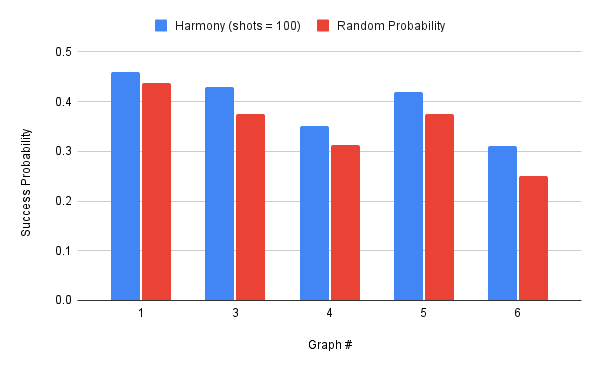
\includegraphics[width=.8\linewidth]{100shotGraph.png}
   \caption{100 shot}
   \label{fig:sfig1}
   \end{subfigure}%
   \begin{subfigure}{.5\textwidth}
   \centering
   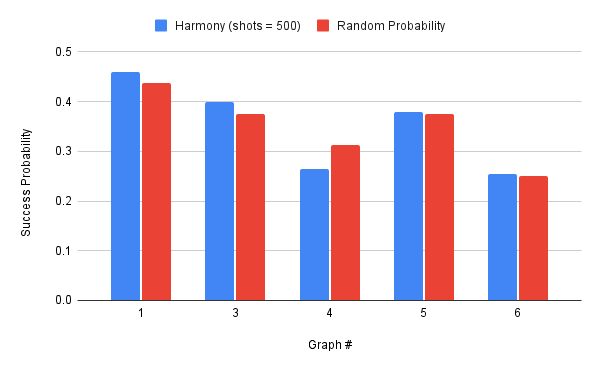
\includegraphics[width=.8\linewidth]{500shotGraph.png}
   \caption{500 shot}
   \label{fig:sfig2}
   \end{subfigure}
   \caption{Success probabilities of Grover's FPS run on IonQ's Harmony with 100 and 500 shots. The measured success probability is shown in blue while the random probability <where eq?> is in red}
   \label{fig:fig}
\end{figure} 

At 100 shots, GFPS has a higher probability of finding the maximal cut than by searching randomly. As the shot number increases to 500, this probability decreases and seems to converge with the random probability for graphs 5 and 6. However, neither of these experiments on harmony display significant increased success probability, that is to say, most advantage that the proposed oracle provides is destroyed by the noise present in NISQ devices.

\medskip
\section{Simulation using small graph}
\label{sec:smallgraphs}
   
\end{comment}

\bigskip

\section{Conclusion}
\label{sec:conclusion}



   %========================
   \bibliography{references}
   %========================

\end{document}